% ch-concentration.tex -- theory: the two concentration models, material properties, boundary conditions
\chapter{濃度と境界条件}
\label{ch:concentration}

モデルについて、説明すべき点があと二つある。溶質の輸送と、計算領域の端での扱いである。どちらも
入力ファイルで選ぶ項目であり、計算コストだけでなく結果そのものを左右する。しかも不用意に選びやすい。
そのため、本章にまとめて説明する。

Yuzenには二つの濃度モデルがある。\val{"WM"}は鉛直一様モデルで、濃度を膜厚方向に一様として扱う。
\val{"CZ"}は膜厚方向の分布を解像する。どちらも一次元と二次元で使える。\val{"WM"}はすべての物理項に
対応するが、\val{"CZ"}では二つの項が使えない。どちらが適切かは一つの無次元数で決まる。この無次元数は
\cref{sec:conc:wm}で示す。

\section{鉛直一様モデル}
\label{sec:conc:wm}

\key{Physics.ConcField.Model = "WM"}では、濃度が膜厚方向に一様であると仮定する。
未知数は各点の$c(x,y,t)$一つだけで、膜厚方向の格子はない。このため計算コストが小さい。
解く方程式は\cref{eq:conc-dim}である。

この仮定が妥当なのは、膜厚方向の拡散が、蒸発で表面から溶媒が失われる速さよりはるかに速い場合である。
つまり、ペクレ数

\[
  \Pen = \frac{E_0 h_0}{D_0}
\]

が小さい場合に限る。低粘度の溶媒からなり、ゆっくり乾燥する薄い液膜であれば、鉛直一様は非常によい近似である。

$\Pen$が小さくないとき、この仮定は成り立たない。しかも、その破綻は特有の形で現れ、結果に大きく影響する。
自由表面付近だけが濃縮され、現実にはそこに硬い皮膜（スキン）ができて、以後の乾燥全体が遅くなる。鉛直一様
モデルはこの現象をまったく表現できない。その結果、次のように誤差が連鎖する。

\begin{itemize}
  \item 皮膜のもとになる膜厚方向の構造がないので、皮膜ができない。そのため、乾燥が遅くなるべきときに遅くならない。
  \item 表面に蓄積するはずの溶質が膜厚全体で平均されるので、表面濃度を\textbf{過小に予測する}。
  \item その結果、\cref{eq:prop-mu}の指数則を低すぎる濃度で評価することになり、粘度の上昇が本来より弱くなる。
  \item マランゴニ応力も弱くなる。マランゴニ応力は表面濃度の勾配で駆動されるが、その勾配が均されているからである。
\end{itemize}

これらは、互いに部分的に打ち消し合うような独立した誤差ではない。いずれも同じ構造の欠如から生じ、
同じ方向に働く。つまり、液膜が現実よりも長く流動性を保つ方向にずれる。

方程式は、各セルの溶質量$hc$の収支として解く。セル界面を横切る溶質は、そこでの濃度に、同じステップで
膜厚の方程式がそのセル界面に流す体積流束を掛けたものとする。そのため、閉じた液膜の溶質量は、蒸発の
有無によらず丸め誤差の範囲で保存される。また、一様な濃度は液膜がどう動いても一様のまま保たれる
（\cref{sec:disc:wm-conservative}）。$c$を$[0, 1]$の範囲に保つには、溶質を切り捨てるのではなく、
セル間で溶質を移動させる（\cref{sec:disc:convection}）。

\key{EnableConvection}と\key{EnableDiffusion}で、対流項と面内拡散項を個別に無効にできる。
テストで一つの機構だけを調べるときに便利だが、物理的に意味のある設定ではない。

\section{\texorpdfstring{\val{"CZ"}}{CZ}モデル：膜厚方向の解像}
\label{sec:conc:cz}

\key{Physics.ConcField.Model = "CZ"}では、膜厚方向を解像して濃度を解く。
解く量は、\key{Grid.Dimension = "xh"}では$c(x,z,t)$、\key{Grid.Dimension = "xyh"}では
$c(x,y,z,t)$である。後者は擬似3次元（pseudo-3D）の場合で、液膜が$x$と$y$に広がり、濃度は
膜厚方向にも解像される。液膜は固定座標$\zeta \in [0,1]$に写像する。そのため、液膜が薄くなると
$\zeta$方向の格子も縮み、膜厚方向のセル数は一定に保たれる。このセル数を\key{Grid.Nz}で与える。

一次元と二次元は同じコードで扱う。液膜の次元は格子で決まり、$N_y = 1$なら$y$の項は一切作らない。
二次元では、膜厚の方程式に$x$--$y$の混合項が、濃度の方程式に$y$--$\zeta$の交差項が加わる。
\file{concz\_2d.toml}を実例として参照されたい。

このモデルの要は$\zeta$方向の境界条件である。濃度の方程式は、$\zeta$格子上で$hc$に
ついての保存形で解く。各セルはセル界面の流束を通じて溶質をやり取りする。$\zeta$方向のセル界面を通る
流束は、液膜のステップに伴う格子の離散的な保存則から決まる。そのため、一様な濃度は一様のまま保たれ、
閉じた液膜の溶質量は丸め誤差の範囲で保存される。基板と自由表面では溶質の出入りはない。そこでは、
蒸発する溶媒による移流と拡散流束全体（表面や基板の傾斜に沿う成分も含む）の和、つまり全流束がゼロになる。
溶媒は溶質を残して最上部のセルから出ていくので、表面付近に濃縮層ができる。蒸発速度は、
膜厚方向の平均ではなく\textbf{自由表面での濃度}で評価する。ここが肝心な点である。これにより、
表面層が自らの乾燥を遅らせるという、鉛直一様モデルにない効果を表現できる。

\begin{figure}[tbp]
  \centering
  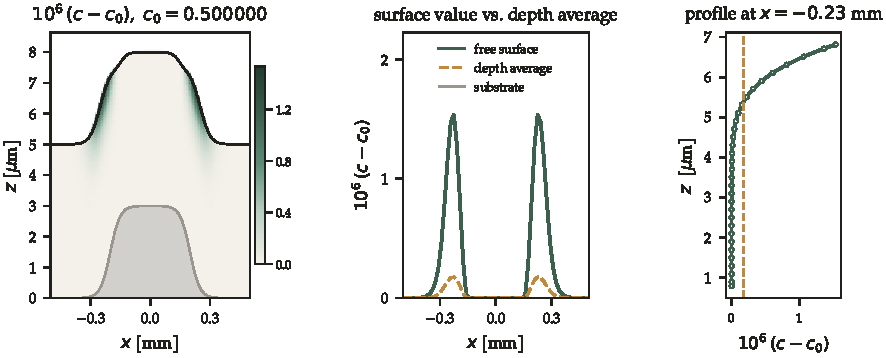
\includegraphics[width=\textwidth]{../figures/concz.pdf}
  \caption{\val{"CZ"}モデルでは解像でき、鉛直一様モデルでは解像できないもの。\file{concz\_2d.toml}の
    計算終了時に、平面$y = 0$上で示す。
    \textbf{左：}基板の起伏の上の液膜。色は$c$から初期値$c_0$を引いた値を表す。
    初期値からのずれは小数第七位に現れる。溶質は自由表面に沿った薄い層に集まっており、それが見えるのは
    二つの肩の部分だけである。\textbf{中央：}$x$方向に沿った、自由表面での値、膜厚方向の平均、基板での値。
    液膜が最も薄い二か所では、同じ蒸発流束がより少ない液体に集中するため、三つの値がはっきり分かれる。
    それ以外の場所では区別できない。
    \textbf{右：}その点での膜厚方向の分布。モデルが用いる$\zeta$格子上で示し、膜厚方向の平均を
    印で示す。鉛直一様の計算で得られるのは破線の値だけである。一方、表面張力と蒸発速度を決めるのは
    実線の最上点である。このケースの\key{Fluid.\bk Diffusivity}は、1-Dのケースの値よりあえて低く
    設定している。元の値に戻すと、拡散によって濃度の段差が半分になる。どこまで下げるかは任意ではなく、
    測定に基づいて決めた。層の深さはおよそ$\sqrt{D t}$であり、セルの高さは\SI{0.2}{\micro\metre}
    だからである。\num{3e-10}では層は四セルにわたり、段差の高さはセル高さに対して二次で収束する。
    二桁低くすると層は一セルより薄くなり、段差の大きさは格子に依存するようになる。具体的な数値は
    ケースファイルに記載している。\label{fig:conc:czprofile}}
\end{figure}

粘度が膜厚方向に変化することから、さらに二つのことが生じる。第一に、面内速度はもはや放物線として解析的に
書けない。そこで、$1/\mu$と$z/\mu$を膜厚方向に数値積分して速度分布を求める。第二に、膜厚は
閉じた形の流束ではなく、この速度分布を膜厚方向に積分したものを流束として進める。これが自由表面での
運動学的条件である。このとき用いる表面張力は、表面濃度での値である。

このモデルにはそれなりのコストがあり、選ぶ前によく検討すべきである。濃度の未知数は$N_x$から
$N_x \times N_z$に増える。さらに重要なのは、使える物理項が減ることである。

\begin{warn}[\val{"CZ"}では分離圧もソース項も使えない]
  \val{"CZ"}で使える項は、毛管圧、溶質マランゴニ効果、鉛直重力、面内重力、遠心力、蒸発である。
  \key{Physics.DisjoiningPressure}と\key{Physics.Source}全体は\textbf{使えず}、
  診断メッセージを出さずに無視される（\cref{sec:ref-physics:disjoining}）。接触線は分離圧によって
  生じるので、\textbf{接触線の問題にはすべて}\val{"WM"}\textbf{を用いなければならない}。
  現在のソルバーでは、膜厚方向に解像した濃度と移動する接触線を組み合わせることはできない。
\end{warn}

\section{物性値の濃度依存性}
\label{sec:conc:properties}

\key{Fluid}ブロックでは、各物性値を基準濃度\key{BaseConc}での値と、そこからの変化則で
与える（\cref{sec:ref-domain:fluidconc}）。

\begin{align}
  \sigma(c) &= \mathrm{BaseValue}
    + \mathrm{Coef}\,(c - \mathrm{BaseConc}),
    \label{eq:prop-sigma}\\
  \mu(c) &= \mathrm{BaseValue}\,
    \exp\bigl(\mathrm{Exponent}\,(c - \mathrm{BaseConc})\bigr),
    \label{eq:prop-mu}\\
  D(c) &= \mathrm{BaseValue}\,
    \exp\bigl(\mathrm{Exponent}\,(c - \mathrm{BaseConc})\bigr).
    \label{eq:prop-diff}
\end{align}

表面張力は濃度の一次関数、粘度と拡散係数は指数関数である。

\Cref{eq:prop-mu}はソルバーの中で最も強い非線形性であり、その強さを具体的に示しておく。
\key{Fluid.Viscosity.Exponent}は10程度になることも珍しくない。この値では、
\textbf{濃度が0.1変化すると粘度は$e$倍になる}。乾燥計算では濃度が十分の数程度変化しうるので、
粘度は桁違いに上昇しうる。これは数値計算上の不都合ではなく、液膜が固化して流れが止まるという
物理そのものである。ただし、乾燥計算の終盤でニュートン反復と時間刻みの制御が最も苦労するのも、
このためである（\cref{ch:convergence,ch:timeintegration}）。

濃度と流れは、複数の経路を通じて双方向に連成している。\Cref{eq:prop-sigma}は二か所に同時に現れる。
傾き\key{Coef}は\cref{eq:q-sc}を駆動するマランゴニ数$\Ma$になり、$\sigma(c)$は
毛管圧項\cref{eq:q-cap}の移動度にも含まれる。そのため、マランゴニ応力を無効にしても、乾燥によって
液膜のレベリングの速さが変わる。粘度は$\mu(c)$を通じて\emph{すべての}流束項に入る。このように、濃度場は
流れを決める。逆に流れは、\cref{eq:conc-dim}の対流と、\cref{eq:conc-adv}の蒸発項を割る膜厚を
通じて、濃度場を決める。二つの方程式は双方向に連成しているので、順に解くのではなく同時に解く。

\section{境界条件の物理的な意味}
\label{sec:conc:boundaries}

膜厚の方程式は四階なので、\textbf{各境界に条件が一つではなく二つ必要である}。境界条件を値で書くのではなく、
名前の付いた種類から選ぶのはそのためである。各名前が条件の対を表す。濃度の方程式は二階であり、
同じ名前から条件を一つ受け取る。種類は\key{Boundary.XminBC.Type}と、同様の三つのキーで
設定する。キーの一覧は\cref{ch:ref-bcout}に、各対を格子上でどう課すかは
\cref{ch:discretization}に示す。以下では、各種類が物理的に何を\emph{表すか}を述べる。

\paragraph{\val{"Symmetry"}} 対称面である。この面を横切るものはなく、形状も濃度もこの面に関して鏡映される。
用途は大きく異なる二つがある。一つは、液滴や液膜の中心を境界に置いて計算コストを半分にすることである。
もう一つは、閉じた壁の代わりに用いることである。既定値はこの種類である。

\paragraph{\val{"Periodic"}} 端を反対側の端につなげる。周期構造をもつ基板上の液膜や、実際には
無限に続くパターンの一波長分を計算する場合に用いる。対になる\emph{両}端に指定しなければならない。
片側だけに指定すると、1-Dでも2-Dでも実行開始前に拒否される。遠心力項と\val{"Periodic"}の端を
組み合わせた場合も同様に拒否される（\cref{sec:ref-bcout:boundary}）。

\paragraph{\val{"Pinning"}} 液体の端を固定する。境界での膜厚を指定し、境界を横切る流れを止める。
濃度には勾配ゼロの条件を課す。膜厚が実際にどの値に保たれるかは\cref{ch:ref-bcout}に記載している。
段差、エッジビード、汚れの線などで液体の端が止められた状況を表す。分離圧を\emph{用いず}、接触線も
解像せずに、端の動かない液膜が得られる点に価値がある。つまり、\cref{sec:wetting:sizing}で述べる
コストを一切かけずに済む。

\paragraph{\val{"FreshInlet"}} 流入境界である。境界での\emph{濃度}を、計算開始時の値に保つ。
膜厚は保たず、組み立てのたびに現在の内部点から計算し直す。したがって、流入する液体の組成は固定され、
膜厚は解に応じて自由に変わる。コーティング工程の上流端に、一定組成の液体が流れ込む状況を表す。
仕組みは\cref{sec:ref-bcout:boundary}に示す。

\paragraph{\val{"Outlet"}} 自由流出である。高階の導関数をゼロとし、境界が形状を押し付けずに
液体が出ていくようにする。計算コストの都合で計算領域を切り詰めた場所で、その先の状況について
本当に情報がない場合に用いる。

どの種類を選んでも共通する点がもう一つある。\key{Substrate}の形状は、液膜と濃度に与えた種類によらず
すべての壁で鏡映される。\val{"Periodic"}の対では、反対側の端から接続される
（\cref{sec:ref-bcout:boundary}）。

\begin{warn}[境界の種類は精度だけでなく結果そのものを変える]
  境界の種類は、小数第三位が違う程度の、互いに交換可能な閉じ方ではない。濡れ広がる液滴が
  \val{"Symmetry"}境界に達すると、壁に突き当たったことになる。液体はそこに溜まって膜厚が増し、
  以後は閉じ込められた液滴として時間発展する。同じ液滴が\val{"Outlet"}境界に達すると、
  そのまま計算領域から出ていく。この二つは、答えの異なる別々の物理問題である。入力ファイルを見ても
  その違いはわからない。種類を選ぶ前に、計算領域の端が物理的に\emph{何であるか}を決めること。
\end{warn}
